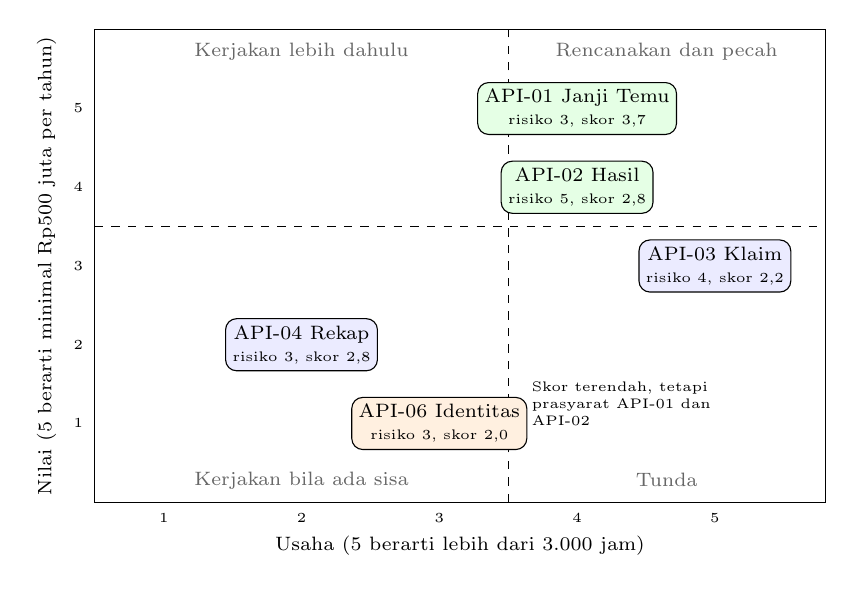
\begin{tikzpicture}[
  x=1.75cm, y=1.0cm,
  font=\scriptsize,
  execute at begin node={\hyphenpenalty=10000\exhyphenpenalty=10000},
  kuadran/.style={font=\scriptsize, text=black!60, align=center},
  terpilih/.style={draw, rounded corners, fill=green!10, align=center, inner sep=2.5pt},
  prasyarat/.style={draw, rounded corners, fill=orange!12, align=center, inner sep=2.5pt},
  antre/.style={draw, rounded corners, fill=blue!8, align=center, inner sep=2.5pt}
]
  % Garis tengah di 3,5 supaya tidak ada kandidat yang tepat di batas kuadran.
  \draw (0.5,0) rectangle (5.8,6);
  \draw[dashed] (3.5,0) -- (3.5,6);
  \draw[dashed] (0.5,3.5) -- (5.8,3.5);

  \node[kuadran] at (2.0,5.72) {Kerjakan lebih dahulu};
  \node[kuadran] at (4.65,5.72) {Rencanakan dan pecah};
  \node[kuadran] at (2.0,0.28) {Kerjakan bila ada sisa};
  \node[kuadran] at (4.65,0.28) {Tunda};

  \foreach \angka in {1,...,5} {
    \node[font=\tiny] at (\angka,-0.2) {\angka};
    \node[font=\tiny] at (0.38,\angka) {\angka};
  }
  \node[font=\scriptsize] at (3.15,-0.55) {Usaha (5 berarti lebih dari 3.000 jam)};
  \node[font=\scriptsize, rotate=90] at (0.15,3.0) {Nilai (5 berarti minimal Rp500 juta per tahun)};

  \node[terpilih] at (4.0,5.0) {API-01 Janji Temu\\{\tiny\mdseries risiko 3, skor 3,7}};
  \node[terpilih] at (4.0,4.0) {API-02 Hasil\\{\tiny\mdseries risiko 5, skor 2,8}};
  \node[antre] at (5.0,3.0) {API-03 Klaim\\{\tiny\mdseries risiko 4, skor 2,2}};
  \node[antre] at (2.0,2.0) {API-04 Rekap\\{\tiny\mdseries risiko 3, skor 2,8}};
  \node[prasyarat] at (3.0,1.0) {API-06 Identitas\\{\tiny\mdseries risiko 3, skor 2,0}};
  \node[font=\tiny, align=left, text width=2.3cm, anchor=west] at (3.6,1.25) {Skor terendah, tetapi prasyarat API-01 dan API-02};
\end{tikzpicture}
